\documentclass[class=minimal,border=0pt,multi=tikzpicture,varwidth=false]{standalone}
%\def\pgfsysdriver{pgfsys-dvisvgm.def}
\usepackage{amsmath}
\usepackage{tikz}
\usetikzlibrary{math}
\usepackage{pgfplots}
\pgfplotsset{width=12cm}
\begin{document}
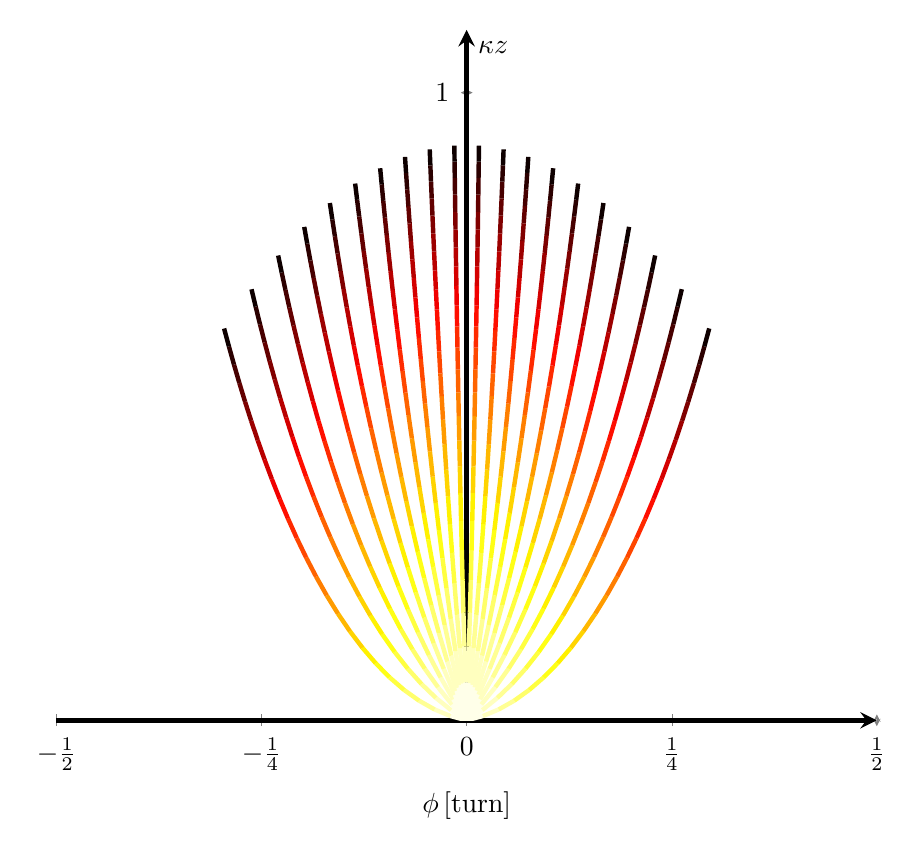
\begin{tikzpicture}[x=1cm,y=1cm]
  \begin{axis}[
      xmin = -2.4675,
      xmax = 2.4675,
      xlabel = {$\phi\,[\text{turn}]$},
      xtick = {-2.4675,-1.2338,0,1.2338,2.4675},
      xticklabels =
        {$-\tfrac{1}{2}$,$-\tfrac{1}{4}$,$0$,$\tfrac{1}{4}$,$\tfrac{1}{2}$},
      axis x line = bottom,
      ymin = 0,
      ymax = 1.1,
      ylabel = {$\kappa z$},
      ytick = {0,1},
      yticklabels = {$0$,$1$},
      axis y line = center,
      ultra thick,
      colormap/hot2,
      every axis/.append style={stealth-stealth}
    ]
    \foreach \w in {-0.95,-0.85,...,0.95}
      \addplot[mesh,domain=0:1.5,->,
        point meta={-abs(sin(deg(x/1.571)))*exp(y)/abs(sin(deg(0.5*\w*pi)))}
        ] (
        {1.571*rad(asin(x*sin(deg(0.5*\w*pi))/sqrt(1+2*x*cos(deg(0.5*\w*pi))+x*x)))}
      , {0.5*ln(1+2*x*cos(deg(0.5*\w*pi))+x*x) } );
  \end{axis};
\end{tikzpicture}
\end{document}
